\section{La Mort aux Trousses}

\subsection*{Introduction}

Suite à la révélation d'un des adversaires des joueurs, le conclave du vampire décide de répondre.
Ce chapitre de l'aventure commence par l'assassinat du principal allié des joueurs.

Ennemi supplémentaire:

L'ombre de Sichua
 - Assassin orphelin sans aucun véritable nom.
 - Sans aucune famille, une seule chose compte lui-même
 - Il veut devenir immortel à tout prix
 - Il est aussi maître chanteur. Il utilise ça surtout contre ses anciens
   employeurs. Il lui arrive aussi de fouiller les documents de ses
   victimes à la recherche de dossiers incriminant pour leur proches.
 - C'est un gros joueur, il laisse pas mal d'argent Aux Dés d'Argent
 - Membre du conseil des cinq

\subsubsection*{Le Conseil des Cinq}

Le groupe est introduit auprès du conseil des cinq. Ceux ci leur demande de 
résumer leurs découvertes.

Les joueurs choisissent un patron parmis les cinq.

\subsubsection*{Choisir sa voie}

Selon le niveau de débrouillardise des joueurs, il faut les pousser plus ou moins.

Il y a trois voies possibles, l'infiltration de la guilde des voleurs, l'infiltration
démonistes (si ils n'ont pas été détruit), l'infiltration des chasseurs de monstres,
les troubles nécromantiques.

\subsection*{L'invasion de morts vivants}

\subsection*{L'infiltration de la guilde des voleurs}

Trouver un voleur pour être introduit auprès de la guilde

-> Dead end les voleurs disparaissent les uns après les autres.

\subsection*{Le Culte Démoniste}

\subsubsection*{Infiltration}
Si ils ne l'ont pas déjà, leur patron fournit l'amulette d'Azazel

\begin{figure}[htb!]
\center
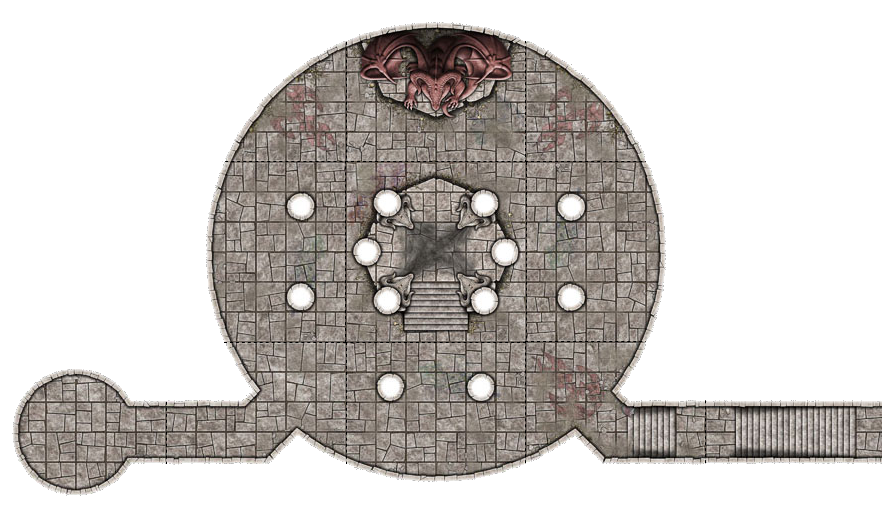
\includegraphics[width=7cm]{Maps/Temple.png}
\end{figure}

Le groupe se rend dans les quartiers où se trouvent le plus de démonistes. 
Alors qu'ils mènent leur enquête, ils sont guidé vers une auberge où se 
trouverait des cultistes. Alors que les joueurs sont dans l'auberge des sons 
étranges résonne dans le bâtiment. Le groupe est alors attaqué par un Vrock
(page \pageref{Vrock}). Lorsqu'ils trouvent le lieu d'origine de la bête, ils trouvent un 
pentacle de sang au sol et quelques cultistes qui se sont apparement saigné 
à mort pour l'invocation.

L'intérogatoire d'un survivant révèle que chaque meneur rassemble un petit 
cercle de fidèles et les dirigeants se regroupe dans une instance plus 
importante. Le groupe devra les infiltrer pour découvrir qui dirige réellement
le culte.

Dans le sous sol d'une auberge (potentielle aquisition du groupe)
Prendre la place d'un meneur -> combattre un Diable à chaines.
Meneur ancien tenancier "???"
Ses patrons "Godrik" "Keltar" "Ernoc"

Description de l'auberge, grande salle ronde au sous sol. A l'étage, les 
chambres sont surtout louée à des cultistes. Chambre principale occupée par le leader.

Participation a une première réunion.
Le groupe est demandeur d'exaction. Conundrum moral. Peuvent executer un comdamné à mort ou autre.
Proposition de duel (un contre un) en fin de réunion (challenge majeur). Les joueurs peuvent attendre une meilleure
occasion hors réunion (il faut ensuite convaincre le culte que la prise de 
pouvoir est légitime: autre combat) ou préparer la rencontre de fin de réunion avec des potions, buffs divers lors de la réunion suivante.


Appel auprès du grand chef. Réunion dans le cimetière du nord. Demande de rassembler des os d'humanoides 
pour une invocation. Ceux qui en ramèneront le plus participeront à l'invocation et gagneront les faveurs de Azazel.
Il sacrifie une jeune femme en fin de réunion sur l'autel.  Occasion en or de l'attrapé isolé.

Options: piller des catacombes ou s'attaquer à une tribu de gobelinoides en marge de la ville et trouver leur cimetière. Il faudra en ramener une carriole!

\subsubsection*{Piller les anciennes catacombes}

Les anciennes catacombes sont vieille de plusieurs siècles, peut être millénaires, elles datent d'une époque où 
les nécromanciens étaient trop nombreux et où il n'était pas raisonnable de conserver des corps 
en grande quantité dans la ville. Les catacombes se trovent à deux jours de marche environ au sud 
de Sichua, le voyage traverse des territoires vallonés et agricoles. Les catacombes se trouvent à
l'auré d'une grande forêt encore sauvage. Les rumeurs sont nombreuses et suffisament effrayante pour
avoir stoppé la progression de la civilisation dans cette direction. Si les joueurs mènent une enquête
dans les alentours sur ces rumeurs, un jet DC 12 en investigation leur permet de s'appercevoir qu'entre
les multiples histoires de fantômes, spèctres, goules et autre morts-vivants, il est aussi souvent 
question d'une sorcière faucheuse d'âmes.

Le patron des aventurier leur fournit une petit cariole avec sa mule et trois barils à remplir 
d'ossements. Un guide connaissant la région les accompagne aussi, malheureusement, celui-ci est
incapable de combattre efficacement (statistiques page \pageref{Eclaireur}). Lorsque le groupe
arrive sur place ils découvrent un ancien temple en grande partie détruit en l'honneur du dieu 
de la mort. Le temple est envahi par la végétation et la forêt alentour est particulièrement
épaisse et impénétrable, il semble impossible d'aller plus loin avec la carriole. Dans les 
décombres du temple derrière l'autel se trouve une arche de pierre avec des runes servant 
d'entrée à un tunnel, c'est très certainement l'entrée des catacombes. Un jet de religion
DC 15 permet d'interpreter ces runes magiques, celles-ci permettent de bloquer le passage
de tout mort-vivant dans un sens ou dans l'autre.

Affrontement de morts vivants qui semblent particulièrement excités.

Fantome en entrant

Arrivé aux catacombes les os semblent s'activer, 6 squeletes et minotaure.
Dans la salle une fouille rapide permet de trouver une lantern of revealing 
sur des ossements plus récents. Probablement ceux d'un pilleur de tombe, la 
lanterne parait intact ce qui attire l'oeil, l'objet semble magique.

Tombe sur une hag qui se considère propriétaire des ossements et compte bien tirer quelque chose des joueurs.
Pendant que ceux-ci visitent la crypte elle tue et remplace le guide des joueurs. Si les joueurs ne voient pas le coup
venir, elle leur pique un objet magique dans la nuit et s'enfuie.

La fouille du corps de la hag permet de trouver plusieurs objets magiques, un anneau de mind shielding
et une Iron flask. Cette dernière si elle est activée révèle une jeune femme appeuré qui déclare
s'appeler Sélia et avoir été enlevé, c'était il y a fort longtemps et elle ne se souvient de rien
de sa vie passé. En fait c'est une succube qui tentera d'user de ses charmes sur l'un des joueurs
masculin de préférence. Si elle est découverte elle tentera de fuir. Elle porte un anneau de regeneration.

Une fouille approfondie des catacombes durant une journée se fait sans rencontre supplémentaire
à l'exceptions de quelques squelettes (combats non joués). Un jet d'investigation DC 15 permet
de trouver un objet d'intérêt. Dans la tombe d'un barde se trouve une mandoline magique
(Canaith Mandolin, Instrument de Barde).

Passage niveau 6.

\subsubsection*{Chasse aux Gobelins}

Affrontement d'une troupe de chasseurs isolés

Combat pour leur ancien lieux de culte 

Poursuite pour échapper

\subsubsection*{Démanteler le culte démoniste}

Au retour en ville le groupe trouve une ville en émois et des combats ont 
lieu dans les faubourgs avec des diables. Après ce combat, les joueurs apprennent
que la garde a du mal a maintenir la paix simplement dans les murs. Les faubourgs 
sont abandonnés aux diables. Lors de la prochaine réunion, il va falloir suivre
quelques leader cultistes et faire du ménage discrètement en attendant le gros 
évenement. Le leader cultiste distribue des parchemins d'invocations.

L'appel vient finalement, rendez vous dans des caves sous les collines du sud.
Un véritable labyrinte ou sont enmené les ossements. Les joueurs sont attaqués
à la sortie par un concurrent mécontent d'avoir été doublé. Si ils suivent un 
autre personnage, il est possible de se débarasser d'une célule démoniste.

Un démon fait du grabuge dans leur quartier d'origine et 
leur biens, voir proches sont en danger. Lorsque les joueurs s'y rendent, ils tombent 
dans un piège de la guilde des assassins. Par chance ceux-ci ne semblent pas avoir 
fait le lien avec leur activités dans le culte diabolique, mais les joueurs vont
devoir rester très attentifs.

Les membres du culte des joueurs demandent une invocation dans leur groupe, car il y
en a eu plusieurs pas loin. Certains membres quittent le groupe pour rejoindre
des voisins. Si les joueurs ne font pas quelque chose, ils reviennent pour les
abattres. Les joueurs peuvent s'attaquer aux voisins, mais attention, il va falloir 
être discret et ne pas se griller dans le culte d'Azazel. Si l'invocation est 
effectuée par l'un des joueurs, sont prochain niveau est automatiquement un 
multiclassage sorcier (si il ne l'et pas déjà) avec Azazel comme patron. (Ce niveau 
pourra être annulé et repris comme un niveau du choix du joueur à la fin du chapitre).

\subsection*{L'invocation}

Les joueurs sont convoqué dans la cave d'une auberge du sud au pied des falaises 
sous la colline ou habite les familles fortunées. La cave de l'auberge s'étend 
sous la colline et les joueurs y trouvent un grand temple qui a été visiblement 
réamenaagé pour le culte d'Azazel. Seul le leader du culte est néanmoins invité à
l'interieur et il doit intervenir avant que ses collègues arrivent pour stopper 
l'invocation. En cas de non intervention un très puissant demon apparait juste 
avant l'arrivée des renforts. Dans ce cas le démon ne sait pas trop à qui faire 
confiance entre les deux camps et décide de massacrer tout le monde.

Les joueurs résté à l'extérieur doivent d'abord combattre quelques cultistes et diables 
pour arriver au temple en toute discrétion et finalement prennent d'assaut le
temple d'Azazel contre une multitude de diables et de cultistes. Le diable majeur étant 
potentiellement présent pour ajouter du chaos à la situation.

En fin de combat, le maitre démoniste est identifié comme étant le maitre des 
golems à la guilde des alchimistes. Ses lettres d'échanges avec le maître assassin
son clair. C'est le chef de la guilde des assassins qui est son principal allié 
et le contact principal avec le maître "sur terre" depuis le départ de Soren vers le 
maître "sous terre". Le dialogue est quelque peu cryptique et clairement cette invocation
interompu devait marqué une prise de pouvoir majeure pour le culte d'Azazel, mais
il reste un membre identifié en ville dont il faut se débarasser et potentiellement
un grand chef qui chapauterait toute cette histoire.

\subsection*{Le Club des Chasseurs}

Contact auprès de la guilde des alchimistes ou de la tour de magie


Identifie le maitre démoniste


